Openflow est un des protocoles qui permet de séparer le plan de données et le plan de contrôle (protocole majoritairement utilisé à l'heure actuelle, étant non propriétaire et porté par l'ONF). Pour l'utiliser, il est nécessaire de disposer de switchs compatibles, c'est à dire des switchs capables de gérer des paquets Openflow. Ainsi, les décisions prises au niveau du contrôleur sont transmises aux switchs concernés par le biais de ce protocole. Pour que l'abstraction de la gestion du réseau soit intéressante, le protocole permet aux switchs une gestion assez fine des paquets reçus à leur niveau, et ce jusqu'au niveau 4 (pour TCP comme on va le voir après). C'est le principal élément de ce qu'on appelle l'interface sud d'un réseau SDN (interface entre contrôleur et entités matérielles) :
\begin{figure}[h]
  	\centering
  	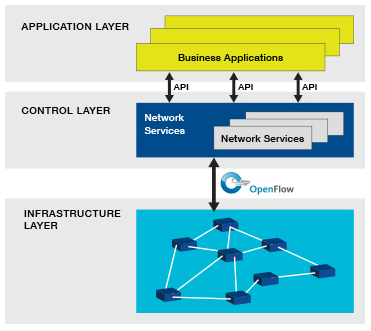
\includegraphics[width=0.45\textwidth]{interfaces.jpg}
  	\caption{Différentes interfaces, Openflow = interface sud}
\end{figure}

Chaque switch (qu'il soit compatible Openflow ou virtuel) consiste en plusieurs tables de flux et une table de groupe (non présente en version 1.0), ainsi qu'un (ou plusieurs) canal(aux) vers le(s) contrôleur(s) (sécurisé(s) via TLS obligatoire en version 1.0 mais obligation supprimée dès la version 1.1 pour des raisons de facilité de déploiement). La description du fonctionnement qui suit est celle de la version 1.3 du protocole (ça n'est donc ni la dernière version, ni la première, mais celle que j'ai principalement utilisée durant le stage, Wireshark la disséquant complètement).\\

La notion de flux est essentielle. Un flux est constitué de 3 parties :
\begin{list}{$\Asteriscus$}{}

\item La première une règle qui filtre les paquets : en fonction des attributs du paquet à l'entrée du switch (port d'entrée physique, adresse ethernet source, adresse ethernet destination, type de paquet, VLAN id, VLAN priority, adresse IP source, adresse IP destination, protocole IP, ToS IP, TCP port source, TCP port destination entre autres). Il est possible de générer des filtrages généraux avec l'utilisation de jokers (wildcard en anglais) sur les champs souhaités (par exemple, si on veut autoriser toutes les adresses ethernet source ayant pour adresse IP x.x.x.x, on pourra utiliser un joker sur le champ adresse ethernet source).

\item La seconde est un compteur qui permet de tenir à jour, si le switch le permet, des statistiques sur l'utilisation du flux.

\item La troisième est une action à appliquer en cas de correspondance du paquet : si le paquet remplit les conditions du filtre, plusieurs types de traitements sont possibles. Entre autres : envoyer le paquet au contrôleur, rediriger le paquet vers un port physique spécifique, vers une table de flux, vers tous les ports sauf le port d'entrée, vers les switchs voisins mis à jour par spanning tree, supprimer le paquet, ou encore modifier certains champs avant redirection, rediriger le paquet vers une queue. Bref, toutes les opérations envisageables sur un paquet. Certaines de ces actions doivent être prises en charge par les switchs Openflow pour que ceux-ci puissent être considérés comme tels. D'autres actions sont optionnelles (par exemple la redirection vers les switchs mis à jour par spanning tree).

\end{list}

Chaque nouveau flux ajouté au switch par le contrôleur l'est dans une table de flux spécifiée. Ainsi, plutôt que d'avoir à organiser relativement la priorité de chaque flux, des regroupements peuvent se faire par table pour factoriser certains traitements. Le switch parcourt chaque table de flux (en considérant le premier flux de chaque table) jusqu'à trouver un filtrage correct pour le paquet. A ce moment, le paquet parcourt et subit les traitements de chacun des flux dans la table trouvée (c'est la notion de pipeline Openflow) jusqu'à ce qu'une action de redirection soit trouvée. La redirection peut également être faite vers une table de flux de priorité inférieure (pour éviter qu'un paquet boucle indéfiniment).

\begin{figure}[h]
  	\centering
  	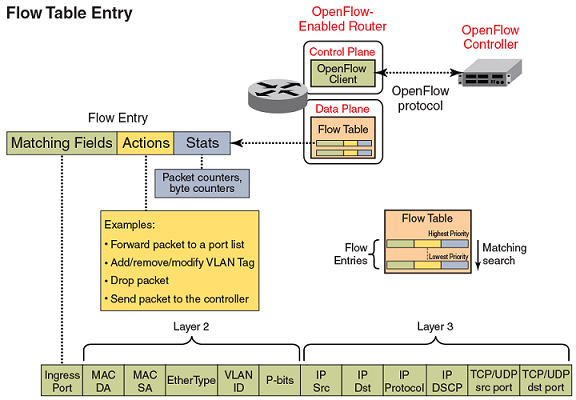
\includegraphics[width=0.9\textwidth]{brocade_flow.png}
  	\caption{Flux et table de flux}
\end{figure}

Basiquement, on peut résumer le protocole Openflow comme étant le protocole permettant :
\begin{list}{$\Asteriscus$}{}

\item de mettre à jour ces tables de flux : ajouts, ajouts partiels (par exemple ajouts de précisions à un flux avec joker), suppressions, modifications, etc ....  

\item d'obtenir des statistiques sur certains éléments (en Openflow 1.3, on peut accéder aux statistiques des flux, des tables, des ports, des queues, des groupes, ou encore du débit (pour la qualité de service)).

\item d'obtenir des informations sur les entités du réseau (nom de l'équipement, nom du fabricant, débit supporté ...)

\end{list}

C'est un protocole qui s'établit de manière classique sur une session TCP (éventuellement surmonté d'une session TLS), habituellement sur les ports 6633 ou 6653 (ce dernier étant maintenant alloué pour cet usage par l'IANA).\\
Il est constitué :

\begin{list}{$\Asteriscus$}{}

\item de messages symétriques (Hello, Echo), qui s'utilisent pour ou démarrer une session Openflow ou s'assurer que les deux parties sont encore connectées

\item de messages contrôleur vers switch (ressemblant à du requête/réponse), généralement les messages qui permettent au contrôleur d'obtenir des informations sur le switchs et de lui donner des ordres. Mais aussi, et c'est important, un message qui permet directement d'insérer du trafic dans le réseau. Ainsi, lorsque le switch envoie un paquet qu'il ne sait pas traiter au contrôleur, celui-ci peut le renvoyer au switch (après l'avoir traité et éventuellement modifié), ce qui évite de perdre le paquet \footnote{On appelle alors ce paquet OFPT\_PACKET\_OUT (selon la spécifiation) qu'on abrégera par la suite en PACKET\_OUT}.

\item de messages asynchrones émis par les switchs, qui sont par exemple susceptibles d'informer le contrôleur lorsqu'ils ont modifié, supprimé ou ajouté un flux, mais également lorsqu'un paquet ne correspond à aucun flux, qu'une erreur survient ou bien qu'un port physique change de configuration. Le message asynchrone le plus important est sûrement celui qui survient lorsque le switch doit envoyer le paquet au contrôleur \footnote{Paquet appelé OFPT\_PACKET\_IN (selon la spécifiation) qu'on abrégera par la suite en PACKET\_IN} (soit parce qu'une règle le demande explicitement, soit parce que le switch ne peut pas traiter le paquet et que la règle par défaut associée demande un envoi au contrôleur).

\end{list}

Ci-dessus une capture Openflow réalisée sous Wireshark.

La figure précédente provient de mes expérimentations, j'ai en effet été amené durant mon stage à créer une sorte de mini-switch virtuel très basique avec Scapy, ce qui m'a forcé à implémenter à la fois la pile TCP et la session Openflow . Même si par la suite cela m'a été peu utile pour réaliser mes scénarios d'attaque, cela m'a permis de bien comprendre le protocole Openflow.

Le lecteur désirant rentrer dans les détails techniques peut se référer à la spécification de la version 1.3\footnote{\label{OF_13}https://www.opennetworking.org/images/stories/downloads/sdn-resources/onf-specifications/openflow/openflow-spec-v1.3.0.pdf (106 pages, dont 49 d'explications)}.